\documentclass[11pt,a4paper,titlepage]{article}
\usepackage[pdftex]{graphicx}
\begin{document}
\begin{figure}
	\centering
	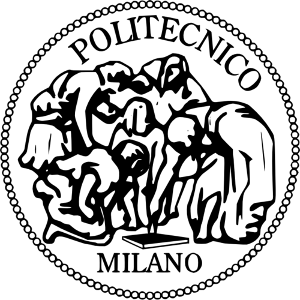
\includegraphics[scale=0.6]{../SE2_IMAGES/Logo_Politecnico_Milano}
\end{figure}
\title{Politecnico di Milano\\A.Y. 2015/2016\\\textbf{My Taxi Service}\\Requirement Analysis and Specification Document\\}
\author{Bernardis Cesare matr. \and Dagrada Mattia matr.852975}
\date{November 6, 2015}
\maketitle

\newpage
\tableofcontents

\newpage

\section{Introduction}

\subsection{Purpose}
The main goal of this document is to completely describe the system in terms of functional and non-functional requirements, to analyse the real need of the customer modelling the system, to show the constraints and the software limits and simulate the typical use cases that will occur after the development. This document is intended to all developers and programmers who have to implement the requirements, to the system analysts who want to integrate other system with this one, and could also be used as a contractual basis between the customer and the developer.
\subsection{Actual system}
The government of a large city wants to optimize its taxi service. We suppose that the actual taxi service is based on simple phone calls from customers to the taxi's call centre.
\subsection{Scope}
The aim of this project is to create a brand new taxi application that is used by both the taxi drivers and the passengers to access the taxi service. Passengers can access the service either via mobile or web application. They can request a taxi without having to register to service but they have to insert personal information while registered passengers, once logged in, can directly request a taxi. The system confirms a taxi request by sending the passenger a code. Registered passengers can also make taxi reservations and they will receive the code 10 minutes before the desired time of the ride. Taxi drivers can access the service only from mobile application. Once logged in they can give the system their availability and will receive from the system ride requests that they can either accept or refuse. The login interface of the application is shared by passengers and taxi drivers.
The system has the city map divided into areas of 2km$^{2}$ and holds taxi queues in each area. It receives GPS coordinates from taxis, it assigns them to their corresponding area queue placing them in the last position. Following a FIFO (First In First Out) logic, the first taxi receives a request that it can accept or refuse. The taxi is removed from the queue and if it refuses the request it is placed in the last position of the queue.
\subsection{Actors}
\begin{itemize}
	\item \textbf{G}uest: a guest is able to request a taxi without having to be registered to the service, but simply adding some essential personal information. A guest can register to the service filling in a registration form, becoming a Registered Passenger.
	\item \textbf{R}egistered \textbf{P}assenger: a registered passenger, once logged in, is able to request a taxi without having to add additional personal information. A registered passenger can also make reservations, specifying origin and destination of the ride, at least 2 hours before the desired time for the ride.
	\item \textbf{T}axi \textbf{D}rivers: a taxi driver, once logged in, has a different user interface than registered user, from which he will receive ride requests that he can accept or refuse. He will also be able to give his availability, which means that he is willing to pick up ride requests.
\end{itemize}
\subsection{Goals}
These are the goals of MyTaxiService application:
\begin{itemize}
	\item Permit a guest to register to the service.
	\item Permit a guest to request a taxi.
	\item Permit a registered passenger to request a taxi.
	\item Permit a registered passenger to make a reservation.
	\item Permit a taxi driver to give the system their availability.
	\item Permit a taxi driver to accept or refuse a ride request.
\end{itemize}
\subsection{Reference Documents}
\begin{itemize}
	\item Specification Document: MyTaxiService Project A.Y.2015-2016.
	\item IEEE Std 830-1998 IEEE Recommended Practice for Software Requirements Specifications.
\end{itemize}
\subsection{Document overview}
This document is structured as following:
\begin{enumerate}
	\item \textbf{Introduction}: this section represents a generic description of the project, highlighting actors and goals.
	\item \textbf{Description}: this section gives further informations about the project, focusing more on what are the assumptions made about the software and its constraints.
	\item \textbf{Requirements}: this section lists the requirements of the software, both functional and non-functional ones.
	\item \textbf{Scenarios}: this section shows some typical scenarios.
	\item \textbf{UML Models}: this section contains some typical use cases and class diagrams.
	\item \textbf{Alloy Modelling}: this section contains Alloy code and Alloy worlds.
	\item \textbf{Appendix}: this section contains extra information and also which software and tools has been used to write this document.
\end{enumerate}

\section{Description}
\subsection{Product perspective}
\subsection{User characteristics}
\subsection{Constraints}
\subsubsection{Regulatory policies}
\subsubsection{Hardware limitations}
\subsubsection{Interfaces to other applications}
\subsubsection{Parallel operation}
\subsubsection{Documents related}
\subsection{Assumptions and Depenencies}
\subsubsection{Assumptions}
\subsubsection{Dependencies}
\subsection{Future possible implementation}

\section{Specific Requirements}

\end{document}